\section{Giới thiệu Grafana}
Grafana là một nền tảng mã nguồn mở hỗ trợ mạnh mẽ cho việc theo dõi và đánh giá các số liệu thu thập được. Vì vậy, Grafana có thể được ứng dụng rộng rãi trong nhiều lĩnh vực khác nhau chứ không chỉ riêng công nghệ thông tin. Bất kì lĩnh vực nào có thể thu thập được dữ liệu theo dòng thời gian đều có thể tối ưu trực quan hóa trên Grafana.
Đối với việc quản trị vận hành phần mềm, Grafana là công cụ hỗ trợ mạnh mẽ việc trực quan hóa các chỉ số (ví dụ như cpu, ram, dish, network, iops, session,…) và nhật ký hoạt động được thu thập từ ứng dụng. Nó có thể kết nối được với nhiều nguồn dữ liệu khác nhau như Prometheus, InfluxDB, ElasticSearch và các công cụ cơ sở dữ liệu quan hệ truyền thống. Nhờ vậy mà ta có thể truy vấn, trực quan hóa, cảnh báo và tìm hiểu dữ liệu bất kể chúng được lưu trữ ở đâu, từ đó tạo ra những hệ thống giám sát sinh động, linh hoạt, dễ dàng nắm bắt thông tin và kiểm soát trạng thái của ứng dụng. 

\begin{figure}[H] % places figure environment here   
    \centering % Centers Graphic
    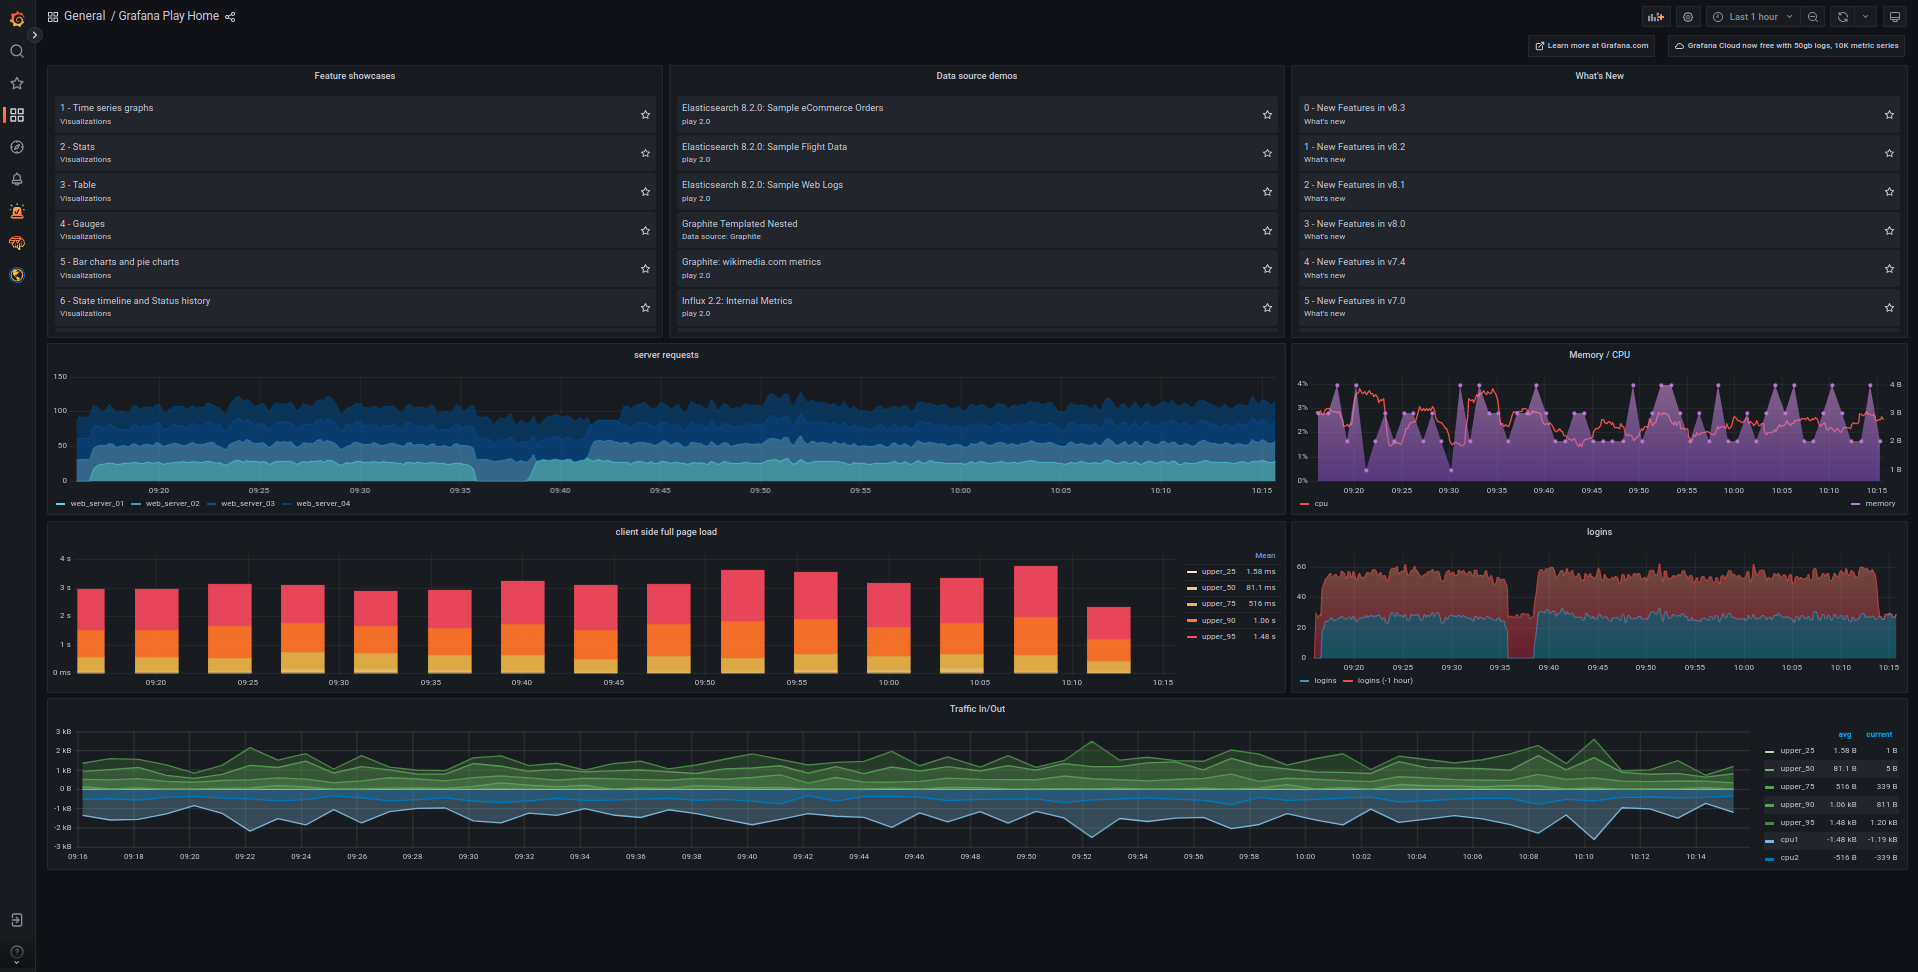
\includegraphics[width=1\textwidth]{figures/fig_01.png} 
    \caption{Một dashboard demo trên trang chủ của Grafana} % Creates caption underneath graph
    \label{fig:fig_01}
\end{figure}

Hình 2.1 thể hiện ví dụ về một dashboard được xây dựng với Grafana. Biểu đồ trên cùng bên trái thể hiện lượng requests tới một website nào đó trong khoảng thời gian một giờ gần nhất. Không chỉ thể hiện tổng lượng request, ta còn có thể quan sát thấy thông lượng tới từng node từ web\_server\_01 đến web\_server\_04 thông qua lớp phủ màu. Ngoài ra khi giữ chuột vào một thời điểm nhất định, biểu đồ cũng cho biết số lượng request cụ thể vào từng node vào thời điểm đó. Biểu đồ trên cùng bên phải thể hiện tài nguyên Memory và CPU được sử dụng của ứng dụng. Các biểu đồ tiếp theo lần lượt đưa ra các chỉ số khác cần theo dõi của ứng dụng.

Grafana có thể ứng dụng với các dashboard trong nhiều lĩnh vực khác nhau, với đa dạng các mục đích. Dưới đây là một số ví dụ minh họa khác về dashboard được xây dựng với Grafana.

\begin{figure}[H] % places figure environment here   
    \centering % Centers Graphic
    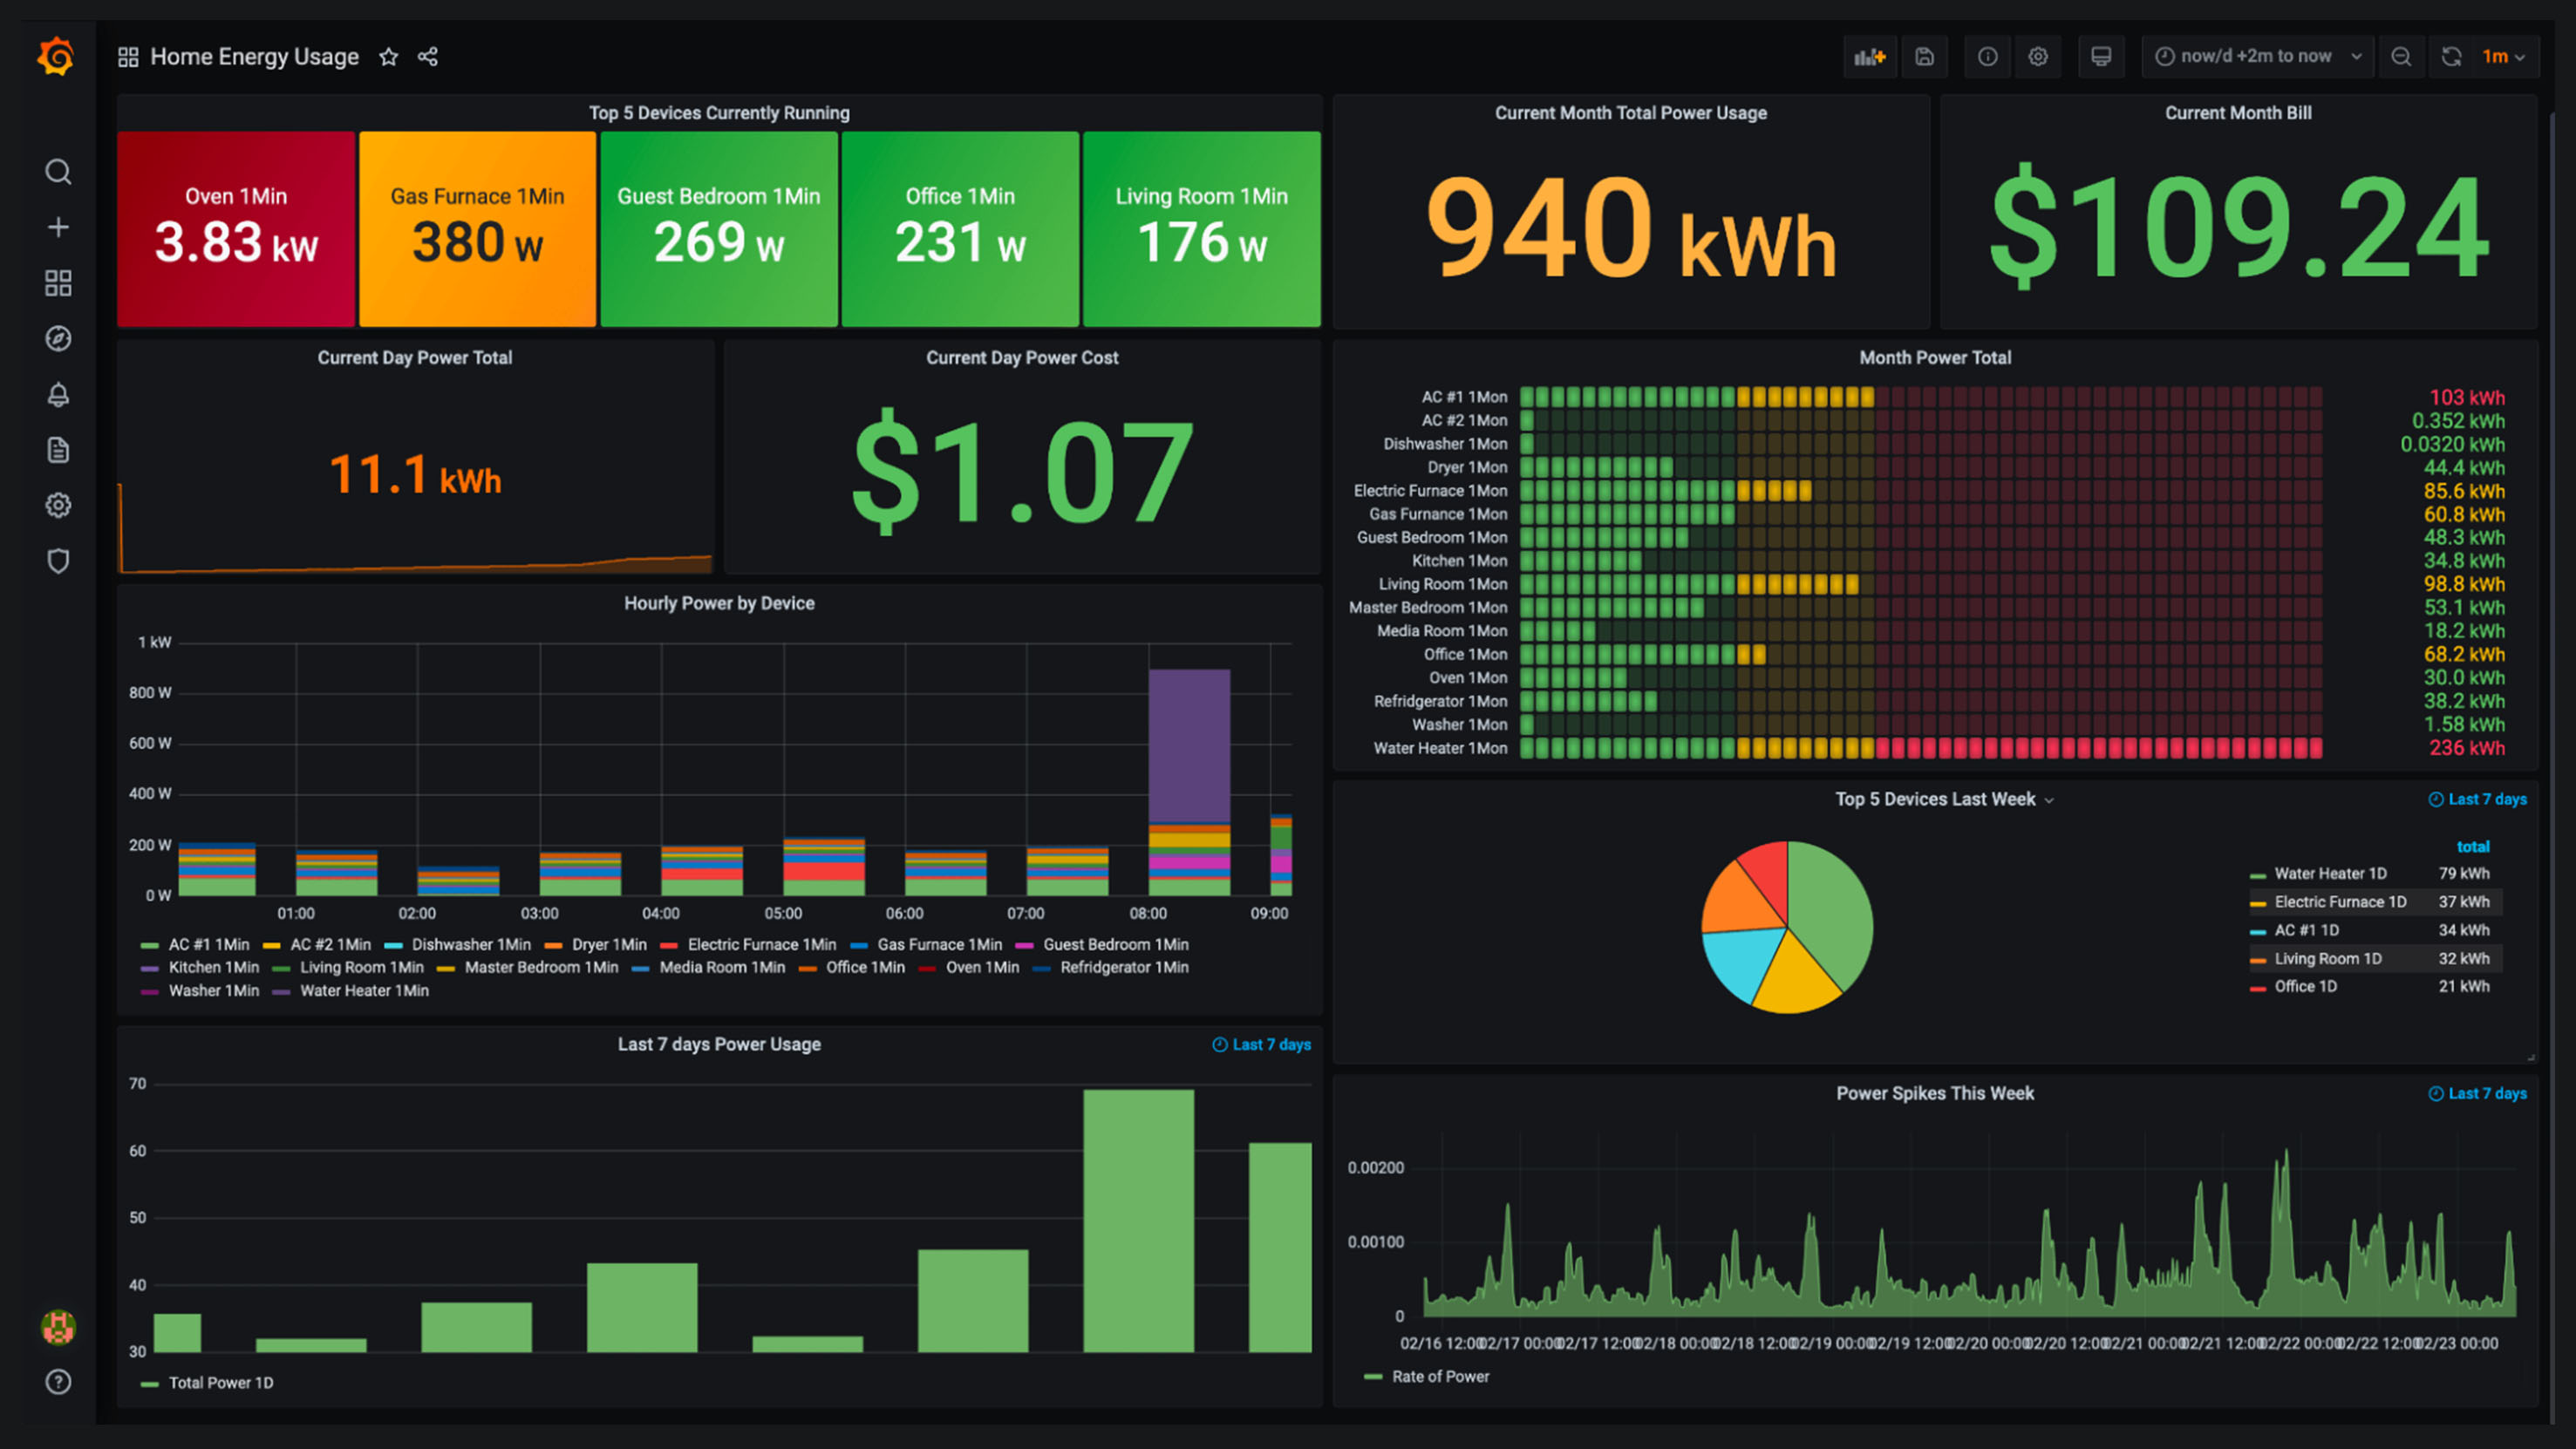
\includegraphics[width=1\textwidth]{figures/Grafana8_HomeEnergy.jpg} 
    \caption{Dashboard đo lường năng lượng tiêu thụ trong hộ gia đình} % Creates caption underneath graph
    \label{fig:fig_01}
\end{figure}

\begin{figure}[H] % places figure environment here   
    \centering % Centers Graphic
    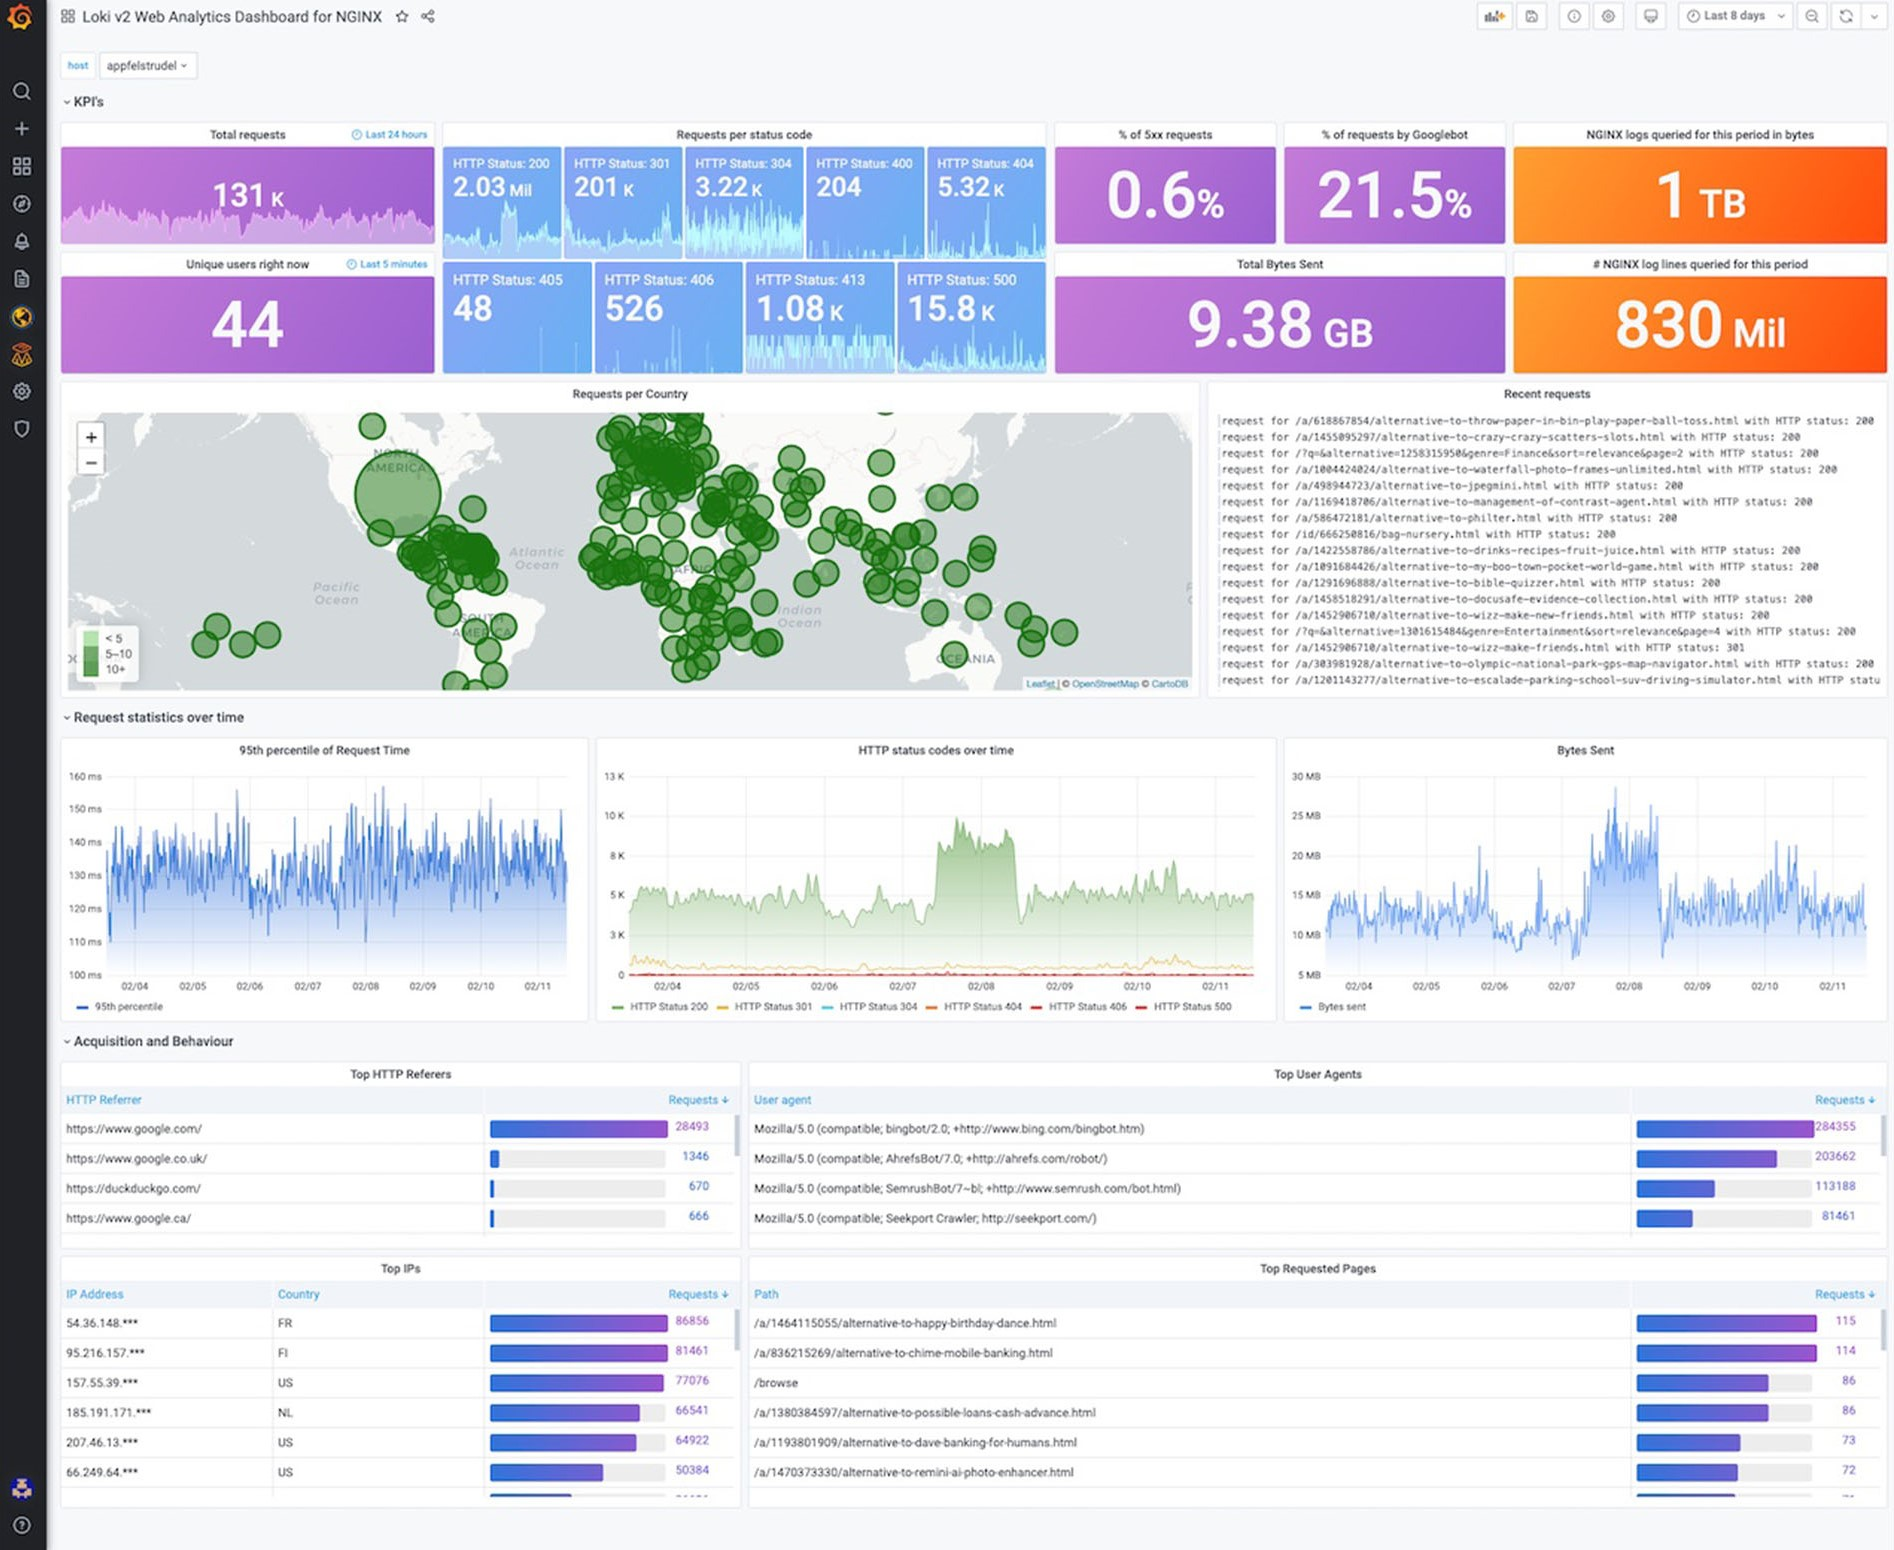
\includegraphics[width=1\textwidth]{figures/Grafana8_WebsitePerformance.jpg} 
    \caption{Dashboard theo dõi hiệu quả của một website} % Creates caption underneath graph
    \label{fig:fig_01}
\end{figure}

\begin{figure}[H] % places figure environment here   
    \centering % Centers Graphic
    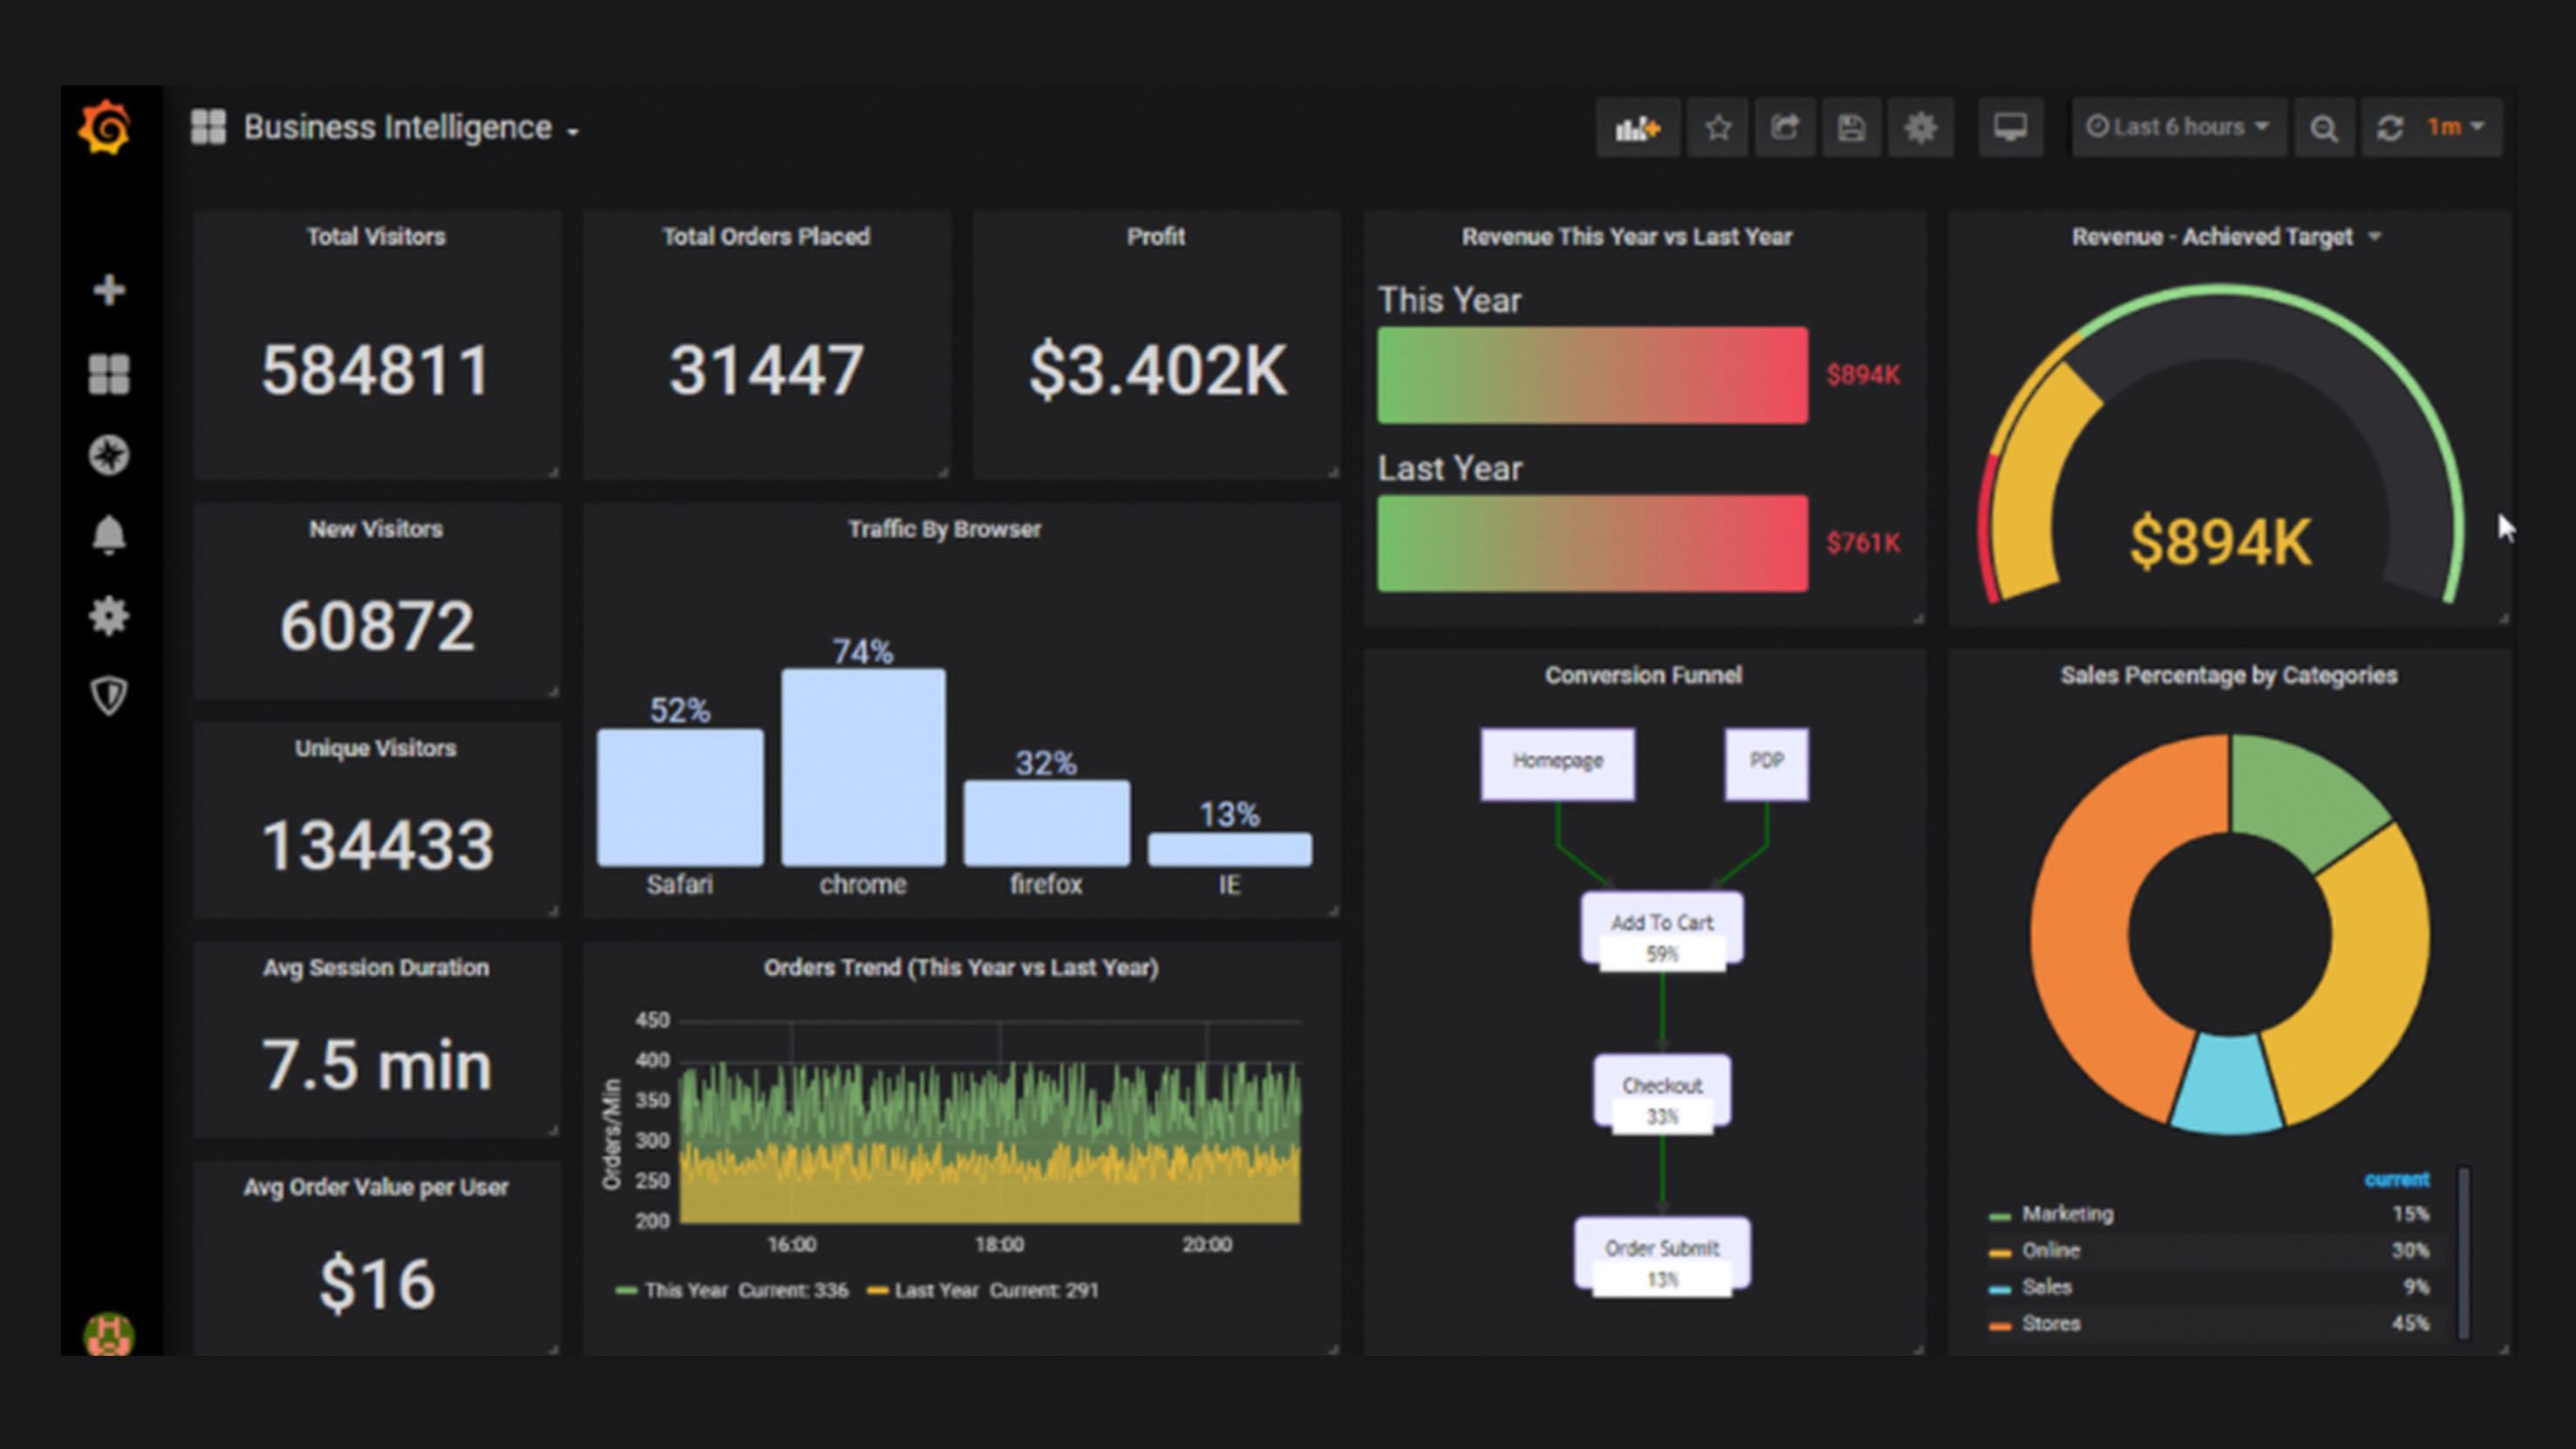
\includegraphics[width=1\textwidth]{figures/Grafana8_Revenue.jpg} 
    \caption{Dashboard theo dõi doanh thu kinh doanh} % Creates caption underneath graph
    \label{fig:fig_01}
\end{figure}

\begin{figure}[H] % places figure environment here   
    \centering % Centers Graphic
    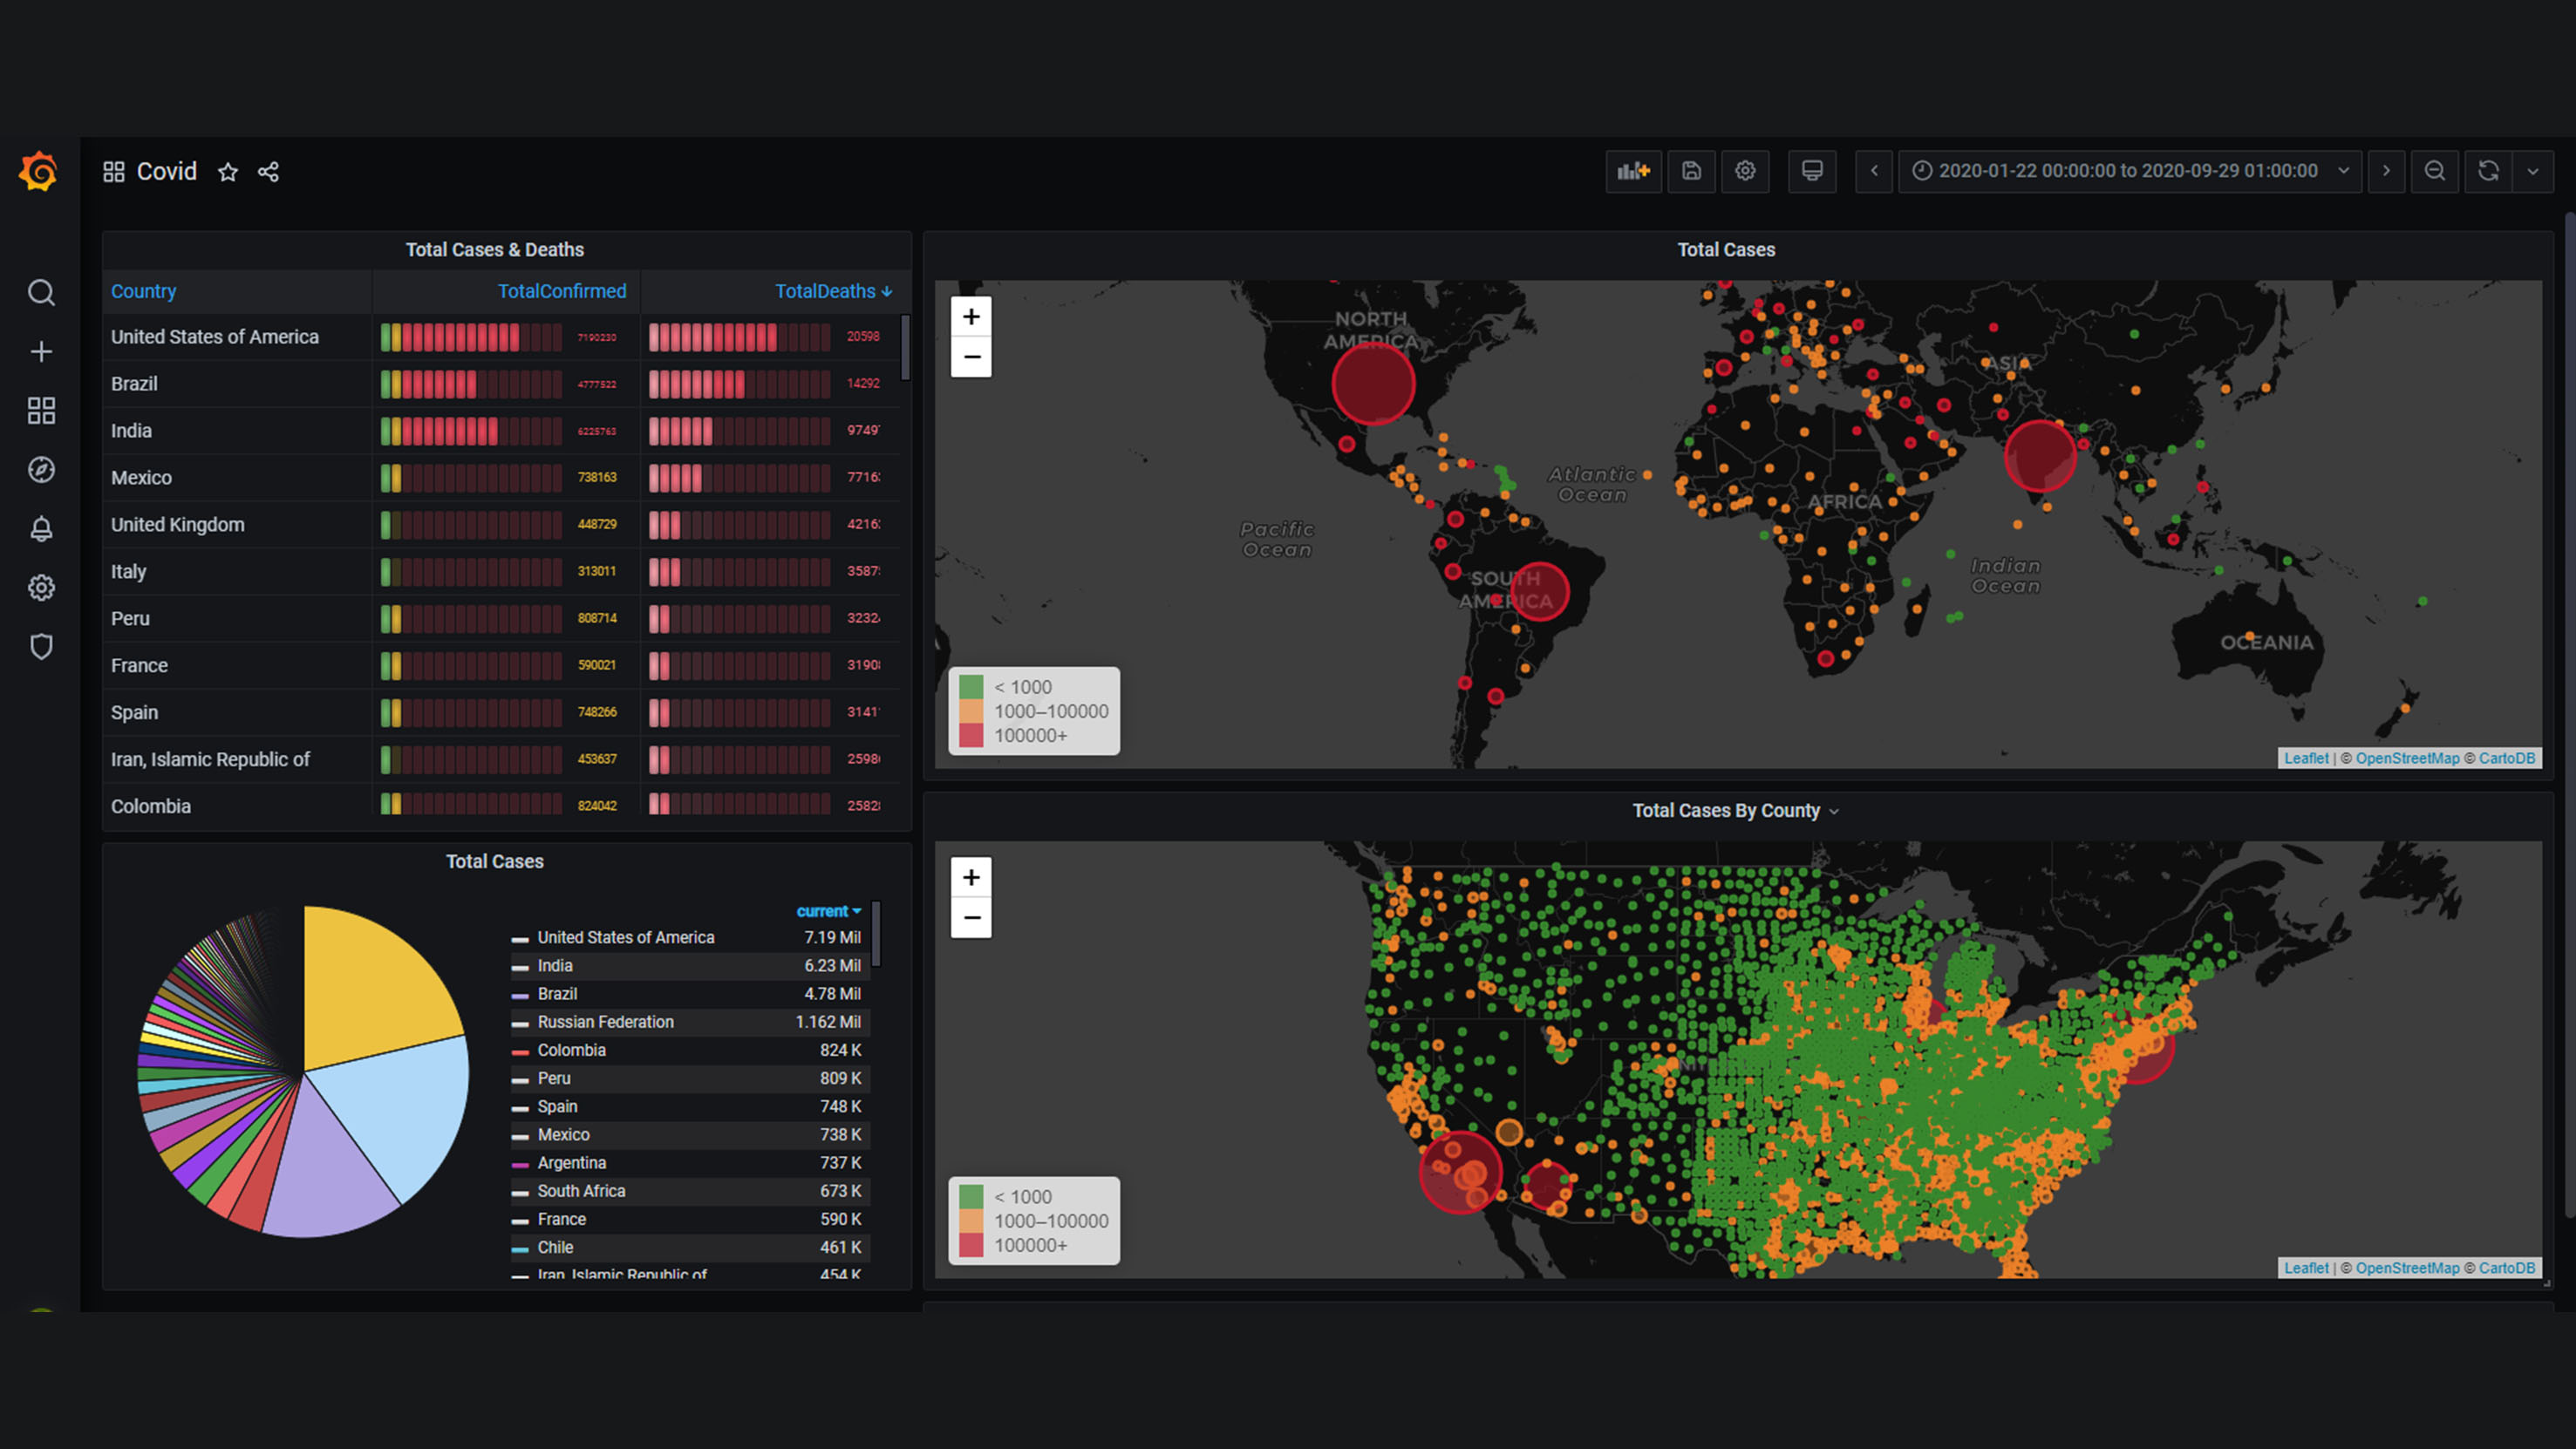
\includegraphics[width=1\textwidth]{figures/Grafana8_Covid19.jpg} 
    \caption{Dashboard theo dõi tình hình dịch bệnh Covid19} % Creates caption underneath graph
    \label{fig:fig_01}
\end{figure}

\begin{figure}[H] % places figure environment here   
    \centering % Centers Graphic
    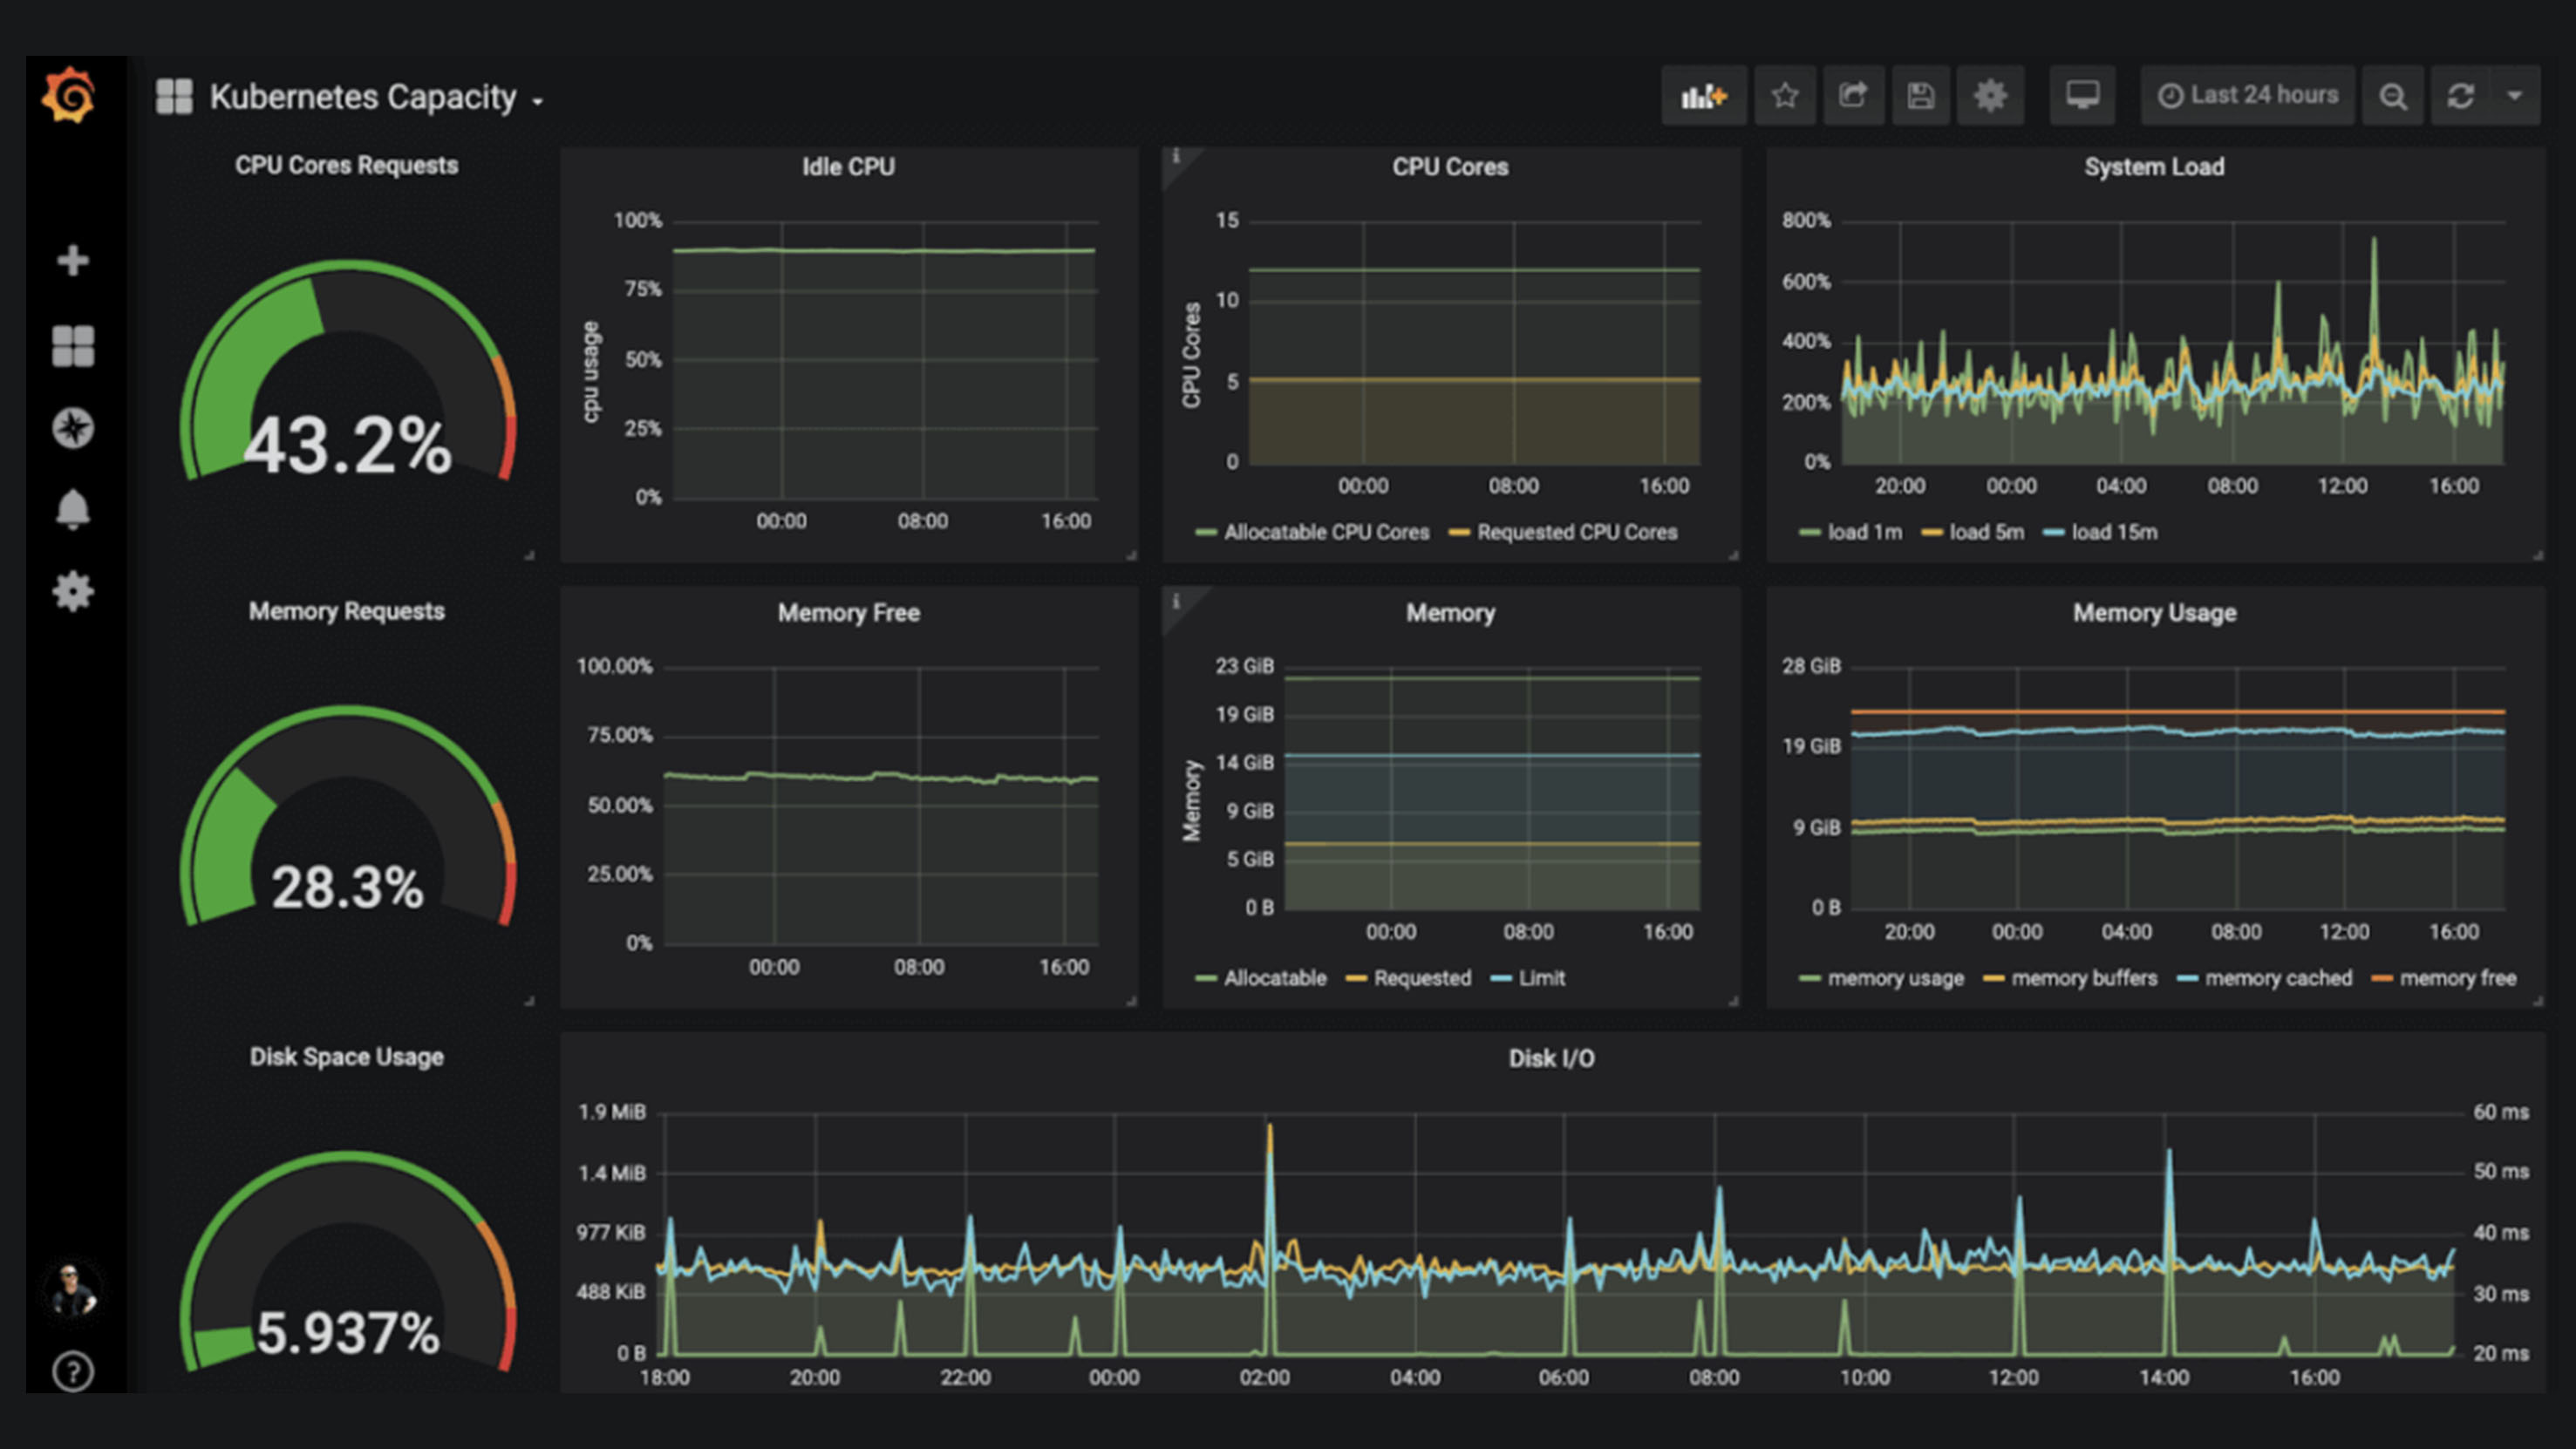
\includegraphics[width=1\textwidth]{figures/Grafana8_Kubernetes.jpg} 
    \caption{Dashboard theo dõi sức chứa hệ thống} % Creates caption underneath graph
    \label{fig:fig_01}
\end{figure}
